\documentclass[11pt,a4paper]{article}
\usepackage[utf8]{inputenc}
\usepackage{graphicx}
\usepackage{minted}

\title{micro:bit LF}
\author{TTK4235}
\date{Kolbjørn Austreng (2018)}

\begin{document}
\maketitle
\section{Oppgave 1: GPIO}
Før dere gir løsningen til studentene, spør dem om spørsmålene i oppgaveteksten for å se om de har lest databladet riktig.
\begin{itemize}
\item Knapp A er koblet til pinne 17; knapp B er koblet til pinne 26.
\item Når knappene blir trykket, vil pinnen lese lav.
\item nRF51822 har et lineært minnekart inndelt i 8 soner. Den første er for kode, så kommer SRAM-minnet, deretter \textit{peripherals}, og så videre. Se figur \ref{fig::nrf51::memorymap}.
\item Baseadressen til GPIO-modulen er 0x50000000.
\item \verb!__RESERVED1_SIZE__! skal være 120.
\end{itemize}
Grunnen til at \verb!__RESERVED1_SIZE__! blir 120, og ikke 121, som mange kanskje fikk, er følgene: Mellom registrene \verb!DIRCLR! og \verb!PIN_CNF[0]! er et tomt rom - nettopp \verb!RESERVED1!. \verb!DIRCLR! starter på offset 0x51C, mens \verb!PIN_CNF[0]! starter på offset 0x700.\\
\\
Dette betyr at \verb!DIRCLR! \textit{slutter} på offset 0x51F (fordi det tar opp 4 bytes = 32 bits). Altså startet tomrommet \verb!RESERVED1! neste byte, nemlig offset 0x520. Da får vi:
\begin{equation}
700_{16} - 520_{16} = 1792_{10} - 1312_{10} = 480_{10}\,\mathrm{bytes} = 120_{10}\,\mathrm{words}
\end{equation}
Om structen hadde brukt typen \verb!volatile uint8_t! istedenfor \verb!volatile uint32_t!, ville \verb!__RESERVED1_SIZE__! blitt 480. Dette er derimot ikke å anbefale, siden structen da sannsynligvis vil få "hulrom" under kompilering, som vil gjøre at \verb!PIN_CNF[0..31]! får feil offset.
\begin{figure}
\centering
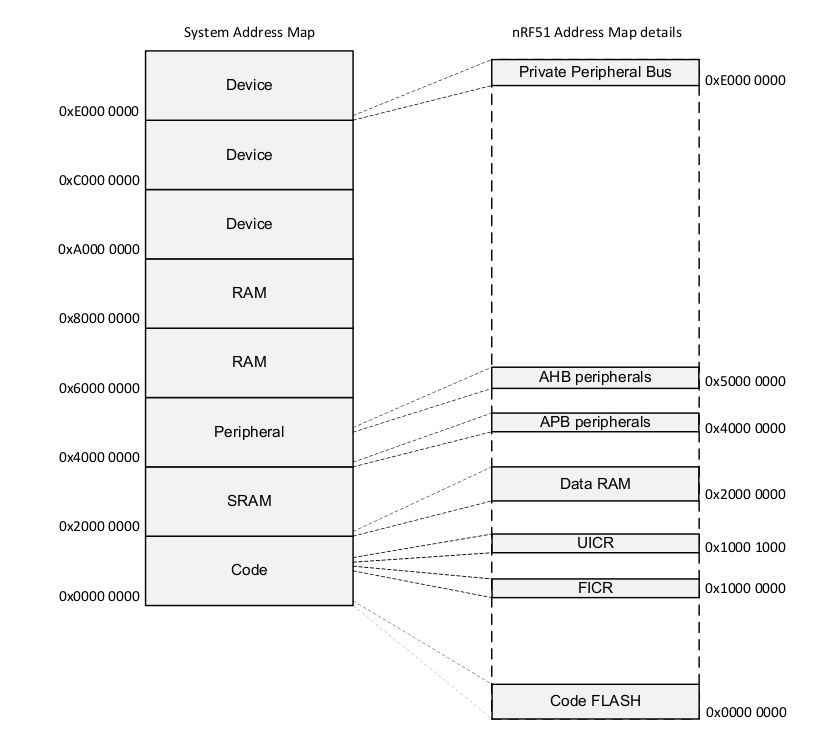
\includegraphics[width=\linewidth]{nRF51memorymap.png}
\caption{nRF51 minnekart.}
\label{fig::nrf51::memorymap}
\end{figure}
\subsection{Referanseimplementasjon}
\inputminted{c}{../build/gpio/main.c}
\subsection{Kommentarer til implementasjon}
\begin{itemize}
\item Koden kan fint splittes opp i for eksempel \textit{main.c} og \textit{registers.h}, uten at makefilen må endres. Dersom studentene dytter hele GPIO-implementasjonen inn i en egen c-fil, må navnet på denne legges til under \mintinline{make}{SOURCES := ...} i makefilen for at den skal kompileres.
\item Om makefilen nekter å kompilere fordi det finnes ubrukte variabler eller tvetydig formatering i koden, så er det på grunn av \mintinline{c}{CFLAGS += -Werror}, som gjør om alle advarsler til feil. Dette er i et forsøk på å tvinge frem pen kode. Dere kan være av en annen oppfatning, så da vet dere hva dere kan fjerne.
\item Navnene på medlemsvariablene i \mintinline{c}{NRF_GPIO_REGS} er helt likegyldig. De kan kalles hva som helst så lenge de refereres til med samme navn senere i koden. Jeg ga dem samme navn som de har i databladet.
\item Strengt talt er det ikke nødvendig med \mintinline{c}{volatile} foran structmedlemmene, fordi hver gang vi kaller \mintinline{c}{GPIO->REGISTER}, får vi en ny instans av \mintinline{c}{NRF_GPIO_REGS}. Dette gjør at kompilatoren ikke kan "optimalisere i stykker" koden vår. Allikevel har jeg tatt med \mintinline{c}{volatile} for kodekvalitetens skyld - for å understreke at medlemsvariablene peker til fysiske registre, som kan endre seg uten at programmet gjør noe.
\item Knappene, \mintinline{c}{GPIO->PIN_CNF[17]} og \mintinline{c}{GPIO->PIN_CNF[26]} må settes til 0; det er ikke nok å sette bare retningsflagget til 0. Dette er fordi de konfigureres som input - og da må vi også koble til inputbufferen. Faktisk kobler Nordic-kode på inputbufferen til ut-GPIO også. En kommentar på Nordic Devzone fra 2014 mente dette kanskje var en bug, men den var der forsatt, da jeg skrev dette.\\
Stort sett virker det som om inputbufferen kan være tilkoblet hele tiden under System ON, men kan kobles fra under System OFF for å hindre flytende IO, og dermed også redusere strømforbruket.
\item \mintinline{c}{main()} har returtype \mintinline{c}{int}. \mintinline{bash}{arm-none-eabi-gcc} vil kompilere "\mintinline{c}{void main()}" om advarsler ikke gjøres om til feil, men \mintinline{c}{int} er i henhold til ANSI- og ISO-standarden for C.
\item Det spiller ingen rolle hva som returneres fra \mintinline{c}{main()}. Den evige løkken burde forhindre at vi kommer dit. Om vi allikevel på en eller annen måte skulle komme dit, så vil vectortabellen tolke det som en feil og resette mikrokontrolleren.
\end{itemize}

\section{Oppgave 2: UART}
Det Nordic kaller "tasks" og "events" er også bare registre. 0 på LSB i disse registrene betyr henholdsvis "ikke utfør task" og "event har ikke skjedd". Grunnen til at de kalles \textit{tasks} og \textit{events} er fordi de kan kobles inn i PPI-modulen og direkte lage et hendelsesorientert system uten at CPUen trenger å være på. Vi kan derimot bruke dem direkte, ved å enten skrive 1 til LSB i tasks-registrene, eller ved å sjekke verdien i et events-register.
\begin{itemize}
\item \mintinline{c}{TGT_TXD} er koblet til GPIO nummer 24.
\item \mintinline{c}{TGT_RXD} er koblet til GPIO nummer 25.
\end{itemize}

\subsection{Referanseimplementasjon}
\subsubsection{uart.c}
\inputminted{c}{../build/uart/uart.c}

\subsubsection{Sende: main.c}
\inputminted{c}{../build/uart/main_tx.c}

\subsubsection{Mottak: main.c}
\inputminted{c}{../build/uart/main_rx.c}

\subsubsection{Frivillig oppgave: main.c}
\inputminted{c}{../build/uart/main_voluntary.c}

\section{GPIOTE}
\subsection{Referanseimplementasjon}
\inputminted{c}{../build/gpiote/}

\end{document}